% --------------------------------------------------------------------------------------------
%
% Author: Brianna Blain-Castelli and Nikkolas Irwin
% Purpose: Project Part 2, CS 620 - HCI
% Date: November 1, 2019
%
% --------------------------------------------------------------------------------------------

\documentclass[11pt]{article}

\usepackage[margin=1in]{geometry}
\usepackage[utf8]{inputenc}
\usepackage[english]{babel}
\usepackage[linktoc=all]{hyperref}
% \usepackage{indentfirst}
\usepackage{titlesec}
\usepackage{tocloft}
\usepackage{setspace}
\usepackage{enumitem}
\usepackage{float}
\usepackage{fancyhdr}
\usepackage{lmodern}
\usepackage{tabularx}
\usepackage{array}
\usepackage{parallel}
\usepackage{lipsum}
\usepackage{graphicx}
\usepackage[dvipsnames, table]{xcolor}
\renewcommand{\cftsecleader}{\cftdotfill{\cftdotsep}}
\newcommand\sectionbreak{\clearpage}

\title{\textbf{Human-Computer Interaction} \\ \Large{CS 420/620} \\ \large{Project Part 2: Requirements Discovery and Specification} \vspace{+16ex}}

\author{\textbf{\Large Team 01} \\ \large{Brianna Blain-Castelli and Nikkolas Irwin}}
\date{\vspace{-2ex} \large{November 1, 2019}}

\begin{document}

\maketitle

\begin{center}
    \vspace{+16ex}
    {\textbf{\Large{Department of Computer Science and Engineering}} \\
    \large{College of Engineering, University of Nevada, Reno} \\
    \large{Course Instructor: Dr. Sergiu Dascalu}}
\end{center}

\pagenumbering{gobble}

\newpage
\pagenumbering{roman}
\tableofcontents
\newpage

\setlength{\cftfigindent}{0pt}  % remove indentation from figures in lof
% \setlength{\cfttabindent}{0pt}  % remove indentation from tables in lot
\listoffigures
% \listoftables

%\doublespacing
\linespread{1.25}
\newpage
\pagenumbering{arabic}
% \singlespacing

%-----------------------------------START-----OF-----SECTION--------------------------------%
\section{Abstract}
\label{sect:abstract}

PyBank, an interactive Python GUI application, simulates a desktop client for personal banking. The application will contain a number of common banking processes such as creating an a new banking account, checking account information, depositing funds, withdrawing funds, and some analytical analysis related to an accounts spending over time. The goal of this application, beyond simulating common banking processes, is to implement principles of human-computer interaction such as the Fundamental Principles of Interaction~\cite{THE_DESIGN_OF_EVERYDAY_THINGS:1} and the Eight Golden Rules of Interface Design~\cite{DESIGNING_THE_USER_INTERFACE:2} so that the application provides an enjoyable experience to its end-users. 

% EOF
%-----------------------------------END-----OF-----SECTION----------------------------------%
\newpage
%-----------------------------------START-----OF-----SECTION--------------------------------%
\section{Requirements Discovery}
\label{sect:requirements_discovery}

Three users were interviewed regarding Pybank to determine what potential users would like to see from this application. The stakeholders who took part in this process were: Chase Carthen, Joseph Masset, and Vinh Le.


%----- START QUESTION 1 ----%
    \bigskip\noindent\textit{"What do you like about any banking or budgeting applications you have seen or utilized yourself?"}
    
    \bigskip\noindent In response to this question, two users both mentioned that they enjoy being able to view their accounts and associated transactions. Chase elaborated that he specifically likes when banks offer options to auto group the transactions as well. On the other hand, Vinh noted the convenience of mobile banking instead, stating that he enjoys being able to scan checks and payments digitally without having to travel to a local bank. 
%----- END QUESTION 1 ------%

%----- START QUESTION 2 ----%
    \bigskip\noindent\textit{"What qualities do you not like about current banking or budgeting application and web clients that you currently use or have seen?"}

    \bigskip\noindent All three users focused on different qualities of applications that they currently utilize. Joseph commented that he dislikes how long it take for data to pool from each location, resulting in inaccuracy of account summaries and transaction details while waiting for the summary to reflect the actual balance. Chase mentioned that he dislikes how functionality for many applications and websites directly employed by banks do not always reflect one another. For this reason, one version may not be able to support use by specific users. Lastly, Vinh responded that the lack of notifications from current banking apps and methods of notification delivery when an alert system is in place can be frustrating. He suggested that notifications for upcoming payments that display directly on a phone or computer would be very useful.
%----- END QUESTION 2 ------%

%----- START QUESTION 3 ----%
    \bigskip\noindent\textit{"If you had the option to have your banking and transaction information displayed visually in a graph, what would you like to see displayed?"}
    
    \bigskip\noindent Two main suggestions were made by the users that were interviewed regarding this application. First, users mentioned that they would find a pie chart or bar graph showing a monthly breakdown of expenditures and budgeting based on transaction purpose to be helpful. Secondly, a line graph that shows income versus expenses per month was recommended in order to visually show successful and less successful saving and profits.
%----- END QUESTION 3 ------%

%----- START QUESTION 4 ----%
    \bigskip\noindent\textit{"What is your favorite type of graph to receive information visually and why?"}
    
    \bigskip\noindent A general consensus was reach by all users that they had a preference for bar graphs and line graphs when looking at financial data. It was stated that, due to clearly marked divisions in categories, it is easy to compare spending of different types when viewing a bar graph. On the other hand, line graphs are better for continuous data and users find their analysis of trends easy to understand.
%----- END QUESTION 4 ------%

%----- START QUESTION 5 ----%
    \bigskip \noindent\textit{"What is the main operating system that you prefer to utilize?"}
    
    \bigskip \noindent All three users interviewed utilize Windows and Linux as their primary operating systems and favor Windows for regular use. For this reason, they expressed interest in the application being compatible with both Windows and Linux; however, in the case that cross-platform functionality cannot be achieved, the users would prefer a Windows client.
%----- END QUESTION 5 ------%

%----- START QUESTION 6 ----%
    \bigskip\noindent\textit{"When utilizing a banking or budgeting application, on average what is the primary function you utilize that it provides? (Ex: Account summaries, transaction details, etc)"}
    
    \bigskip\noindent All three users utilize banking applications with the same primary purpose, to see current account summaries and balances. While individual transaction details and transferring money between accounts were also mentioned in response, they were labelled as secondary to an overall summary of account statuses.
%----- END QUESTION 6 ------%

%----- START QUESTION 7 ----%
    \bigskip\noindent\textit{"Which features do you rarely utilize in banking or budgeting applications?"}

    \bigskip\noindent All three users have different features that they rarely utilize in banking applications, providing different options for deciding priority among functions. Joseph commented that he rarely uses options to follow or graph a budget due to lack of granular control that results in incorrect reporting. Chase instead noted that he does not utilize functions to create spending caps as they are not useful. Lastly, Vinh stated that he does not check his monthly statement on banking applications because it downloads a PDF containing sensitive account information locally to a device. This option is not secure and allows easy access to user information.
%----- END QUESTION 7 ------%    

%----- START QUESTION 8 ----%
    \bigskip\noindent\textit{"When adding a transaction, what information do you find necessary to provide to a banking or budgeting application?"}

    \bigskip\noindent Users responded stating that the most important information to provide are transaction amount, vendor name, account pulled from, and transaction type, such as rent, groceries, or entertainment. Joseph also recommended the addition of an optional notes section that can be regularly edited. This allows the user to include additional details about the transaction that would not typically be provided to better organize why the expenditures are necessary or to create more granular types within the broader spectrum to which the transactions fit. While he has not seen this in practice, he feels it would be a helpful addition to current transaction recording forms.
%----- END QUESTION 8 ------%

%----- START QUESTION 9 ----%
    \bigskip\noindent\textit{"What information are you often asked for when filling forms do you find superfluous?"}
    
    \bigskip\noindent A variety of issues were mentioned surrounding various form fields utilized by banks. In particular, Joseph and Vinh were concerned with personal identifying information that is often requested for the addition of transactions. They expressed that they disliked how much private information needed to be sent to budget and do not view this information as necessary. Chase also mentioned personal information; however, he was frustrated more by the redundancy surrounding this information than privacy. He stated that it is superfluous when banks asks repeatedly for a user’s address on forms when the banks already have this information on file.
%----- END QUESTION 9 -------%

%----- START QUESTION 10 ----%
    \bigskip\noindent\textit{"Is there anything you would like to add?"}

    \bigskip \noindent One user recommended support for various currency types internationally as well as an account option for various cryptocurrencies. This special account type would display information regarding trends in cryptocurrency values and how that value translates into their current holdings similar to stock trading boards. Additionally, the importance of security was mentioned by another user. Extra security is more marketable and will make the service more appealing.
%----- END QUESTION 10 ------%

% EOF
%-----------------------------------END-----OF-----SECTION----------------------------------%
\newpage
%-----------------------------------START-----OF-----SECTION--------------------------------%
\section{Use Cases and HCI Scenarios}
\label{sect:use_cases_and_hci_scenarios}
% Persona 1
\subsection{HCI Persona 1}
\label{sect:hci_persona_1}

\begin{Parallel}[v]{0.48\textwidth}{0.48\textwidth}
\ParallelLText{
\begin{minipage}{0.40\textwidth}
    \begin{figure}[H]
        \begin{centering}
        	\colorbox{lightgray}{{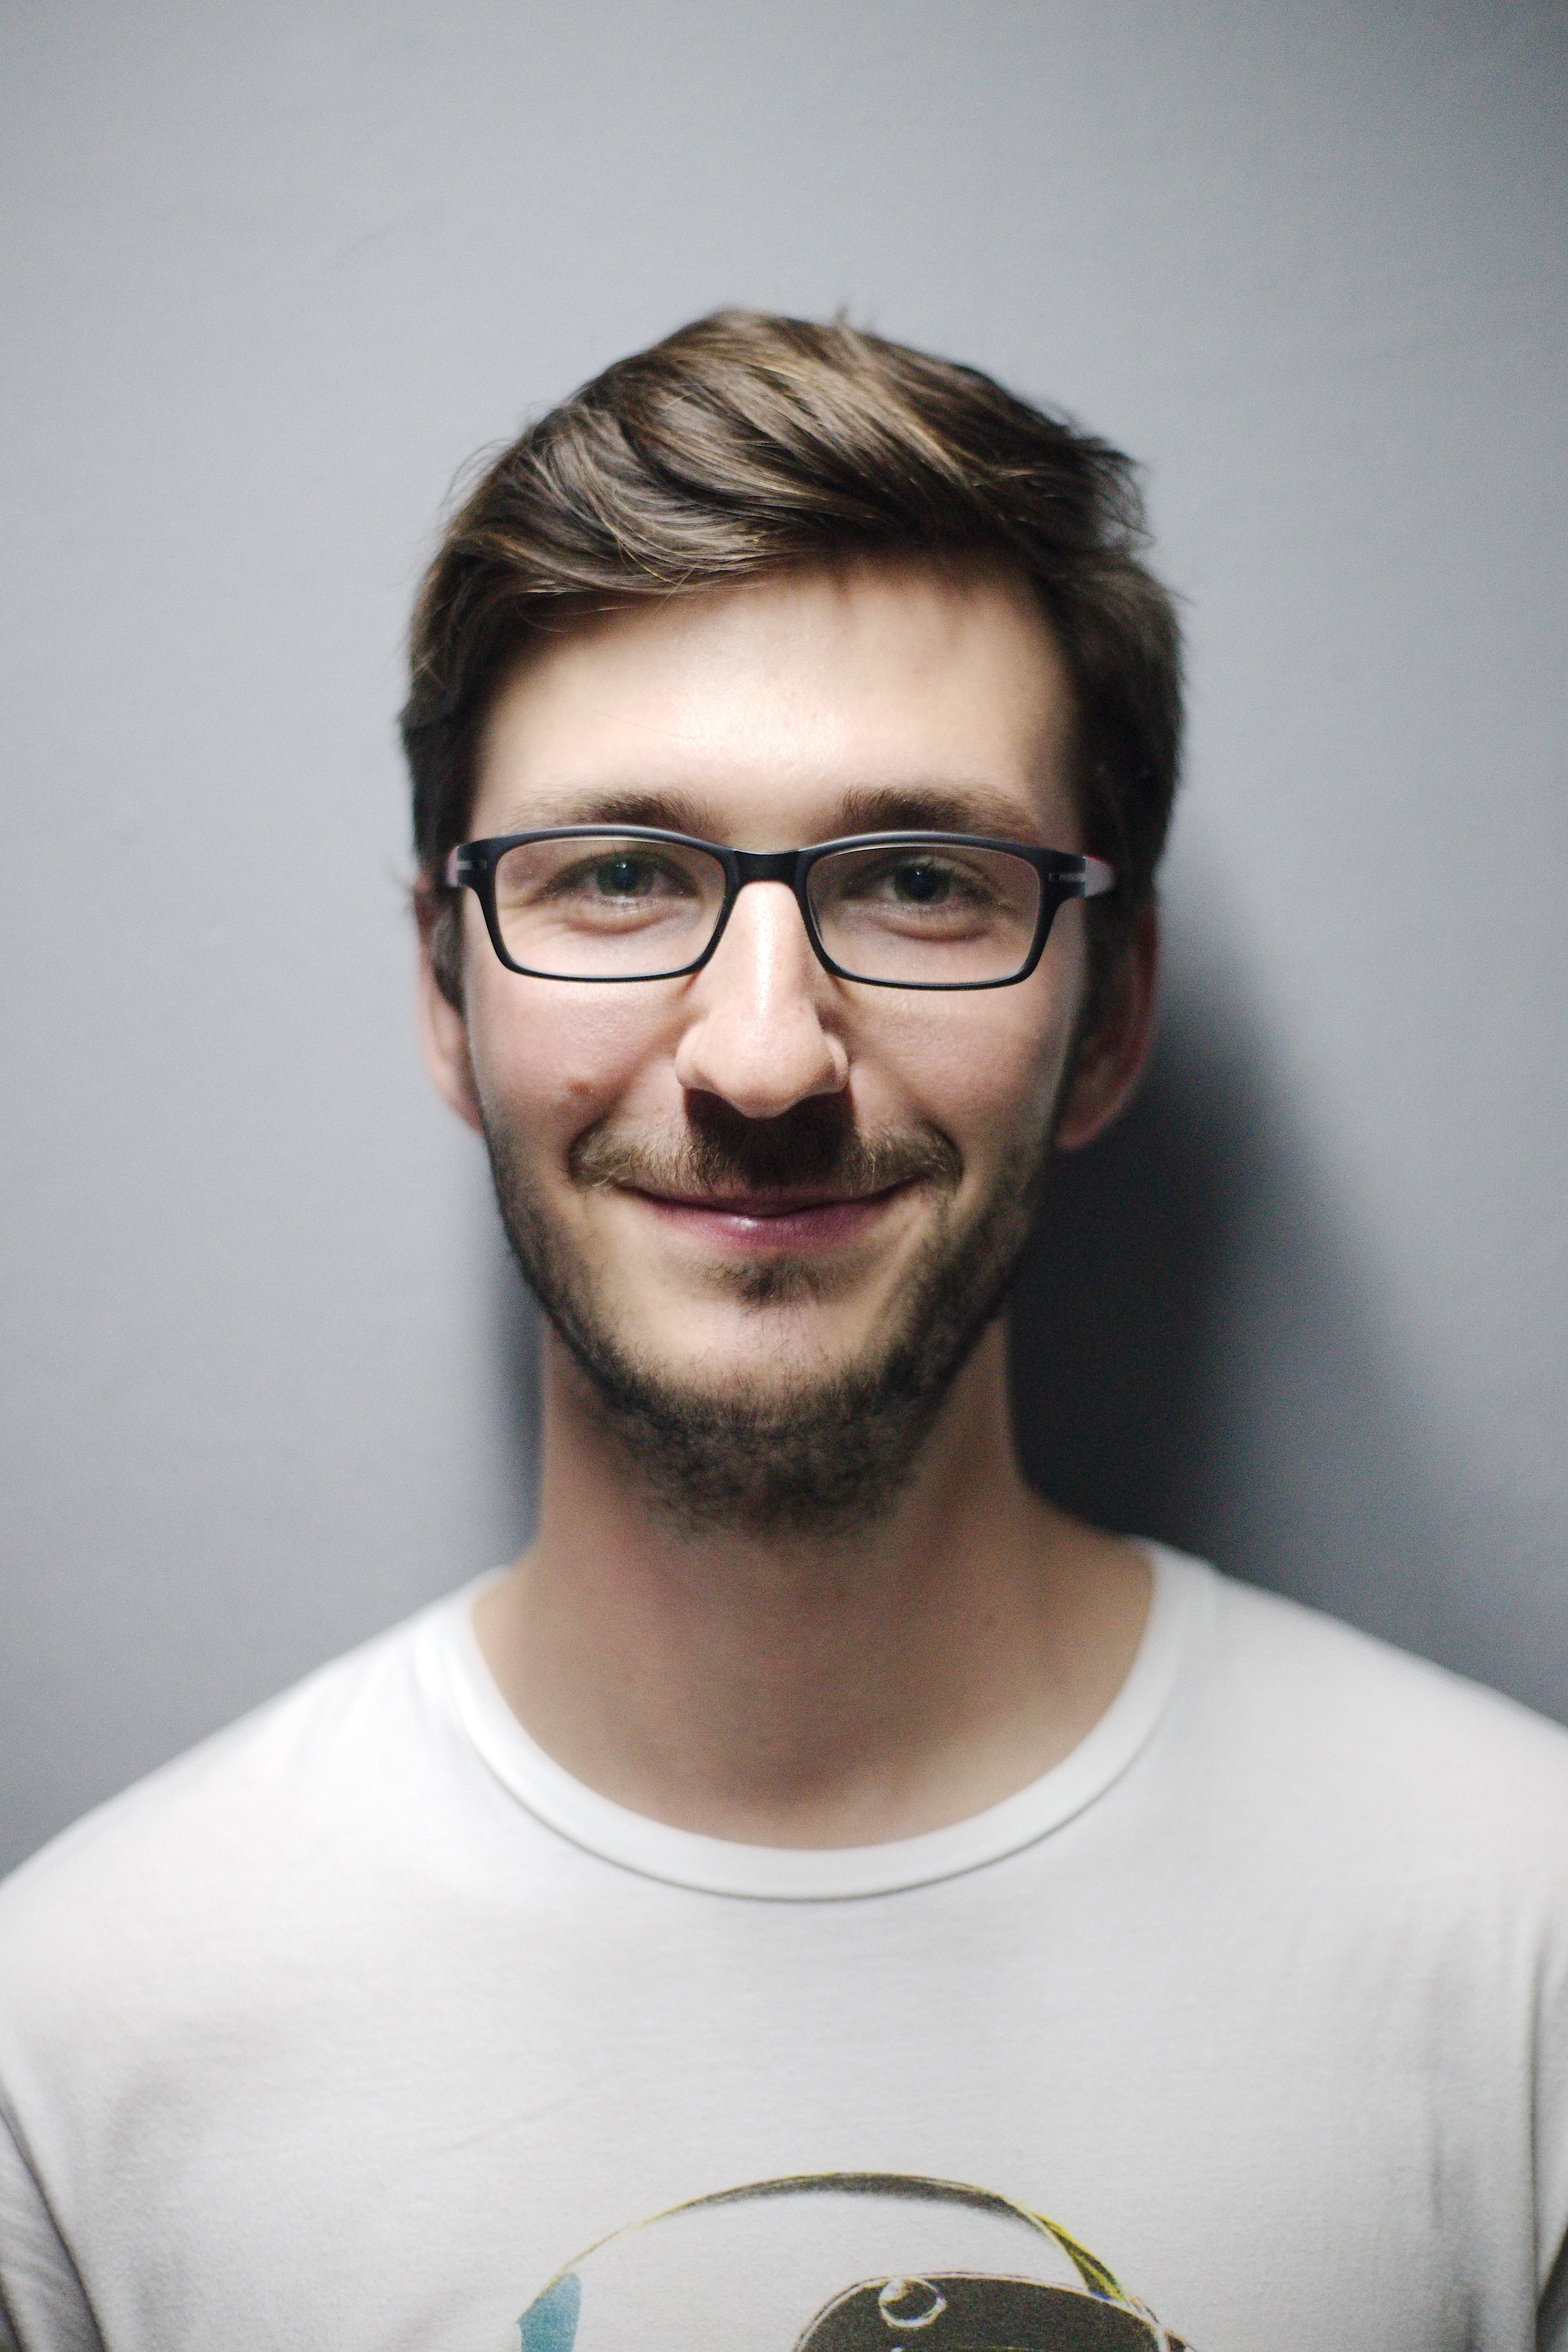
\includegraphics[width=0.80\linewidth, height=1.00\linewidth]{personas/persona_1.jpg}}}
        	\caption{A photo of a fictional male persona for the PyBank application~\cite{PEXELS_MALE_PERSONA:4}.}
        	\label{fig:persona_1}
        \end{centering}
    \end{figure}
    \begin{centering}
        \begin{itemize}[leftmargin=*]
            \item {\textbf{Fictional Name:}~John Doe}
            \item {\textbf{Job Title:}~Accountant}
            \item {\textbf{Demographics:}
                \begin{itemize}[leftmargin=*]
                    \item {\textbf{Age:}~26}
                    \item {\textbf{Marital Status:}~Single}
                    \item {\textbf{Degree:}~B.A. Accounting}
                \end{itemize}
            \item {\textbf{Goals and Tasks:}
                \begin{itemize}[leftmargin=*]
                    \item {Perform accounting services for local companies using PyBank's desktop client.}
                    \item {Learn PyBank's interface in-depth to become a power user.}
                \end{itemize}}}
        \end{itemize}
    \end{centering}
\end{minipage}}
\ParallelRText{\begin{minipage}{0.40\textwidth}
    \subsubsection*{Environment}
    \begin{centering}
        John, an accountant for a local firm, typically performs work on a desktop computer system. He's a busy individual, handling the accounts of both local and widespread businesses. John's spends the majority of his time performing financial computations, answering phones, and writing complex reports with visualizations. Sometimes, when John has to travel, he performs work-related tasks on a laptop computer system instead of other mobile alternatives because he always wants to have the highest performance while working for his clients.
    \end{centering}
    \subsubsection*{Scenario}
    \begin{centering}
        John recently began merging all of his clients accounts into to the PyBank desktop application. During a recent trip, where internet activity was scarce, John was prepared. Thanks to Pybank, John was still able to perform accounting tasks for his clients that were processed, recorded, and once he regained internet access, updated in the cloud. PyBank's flexibility and accessibility allowed John to perform work that other individuals were restricted from performing with traditional banking systems.
        \vspace{10mm}
    \end{centering}
\end{minipage}}
\ParallelPar
\end{Parallel}

\newpage

% Persona 2
\subsection{HCI Persona 2}
\label{sect:hci_persona_2}

\begin{Parallel}[v]{0.48\textwidth}{0.48\textwidth}
\ParallelLText{
\begin{minipage}{0.40\textwidth}
    \begin{figure}[H]
        \begin{centering}
        	\colorbox{lightgray}{{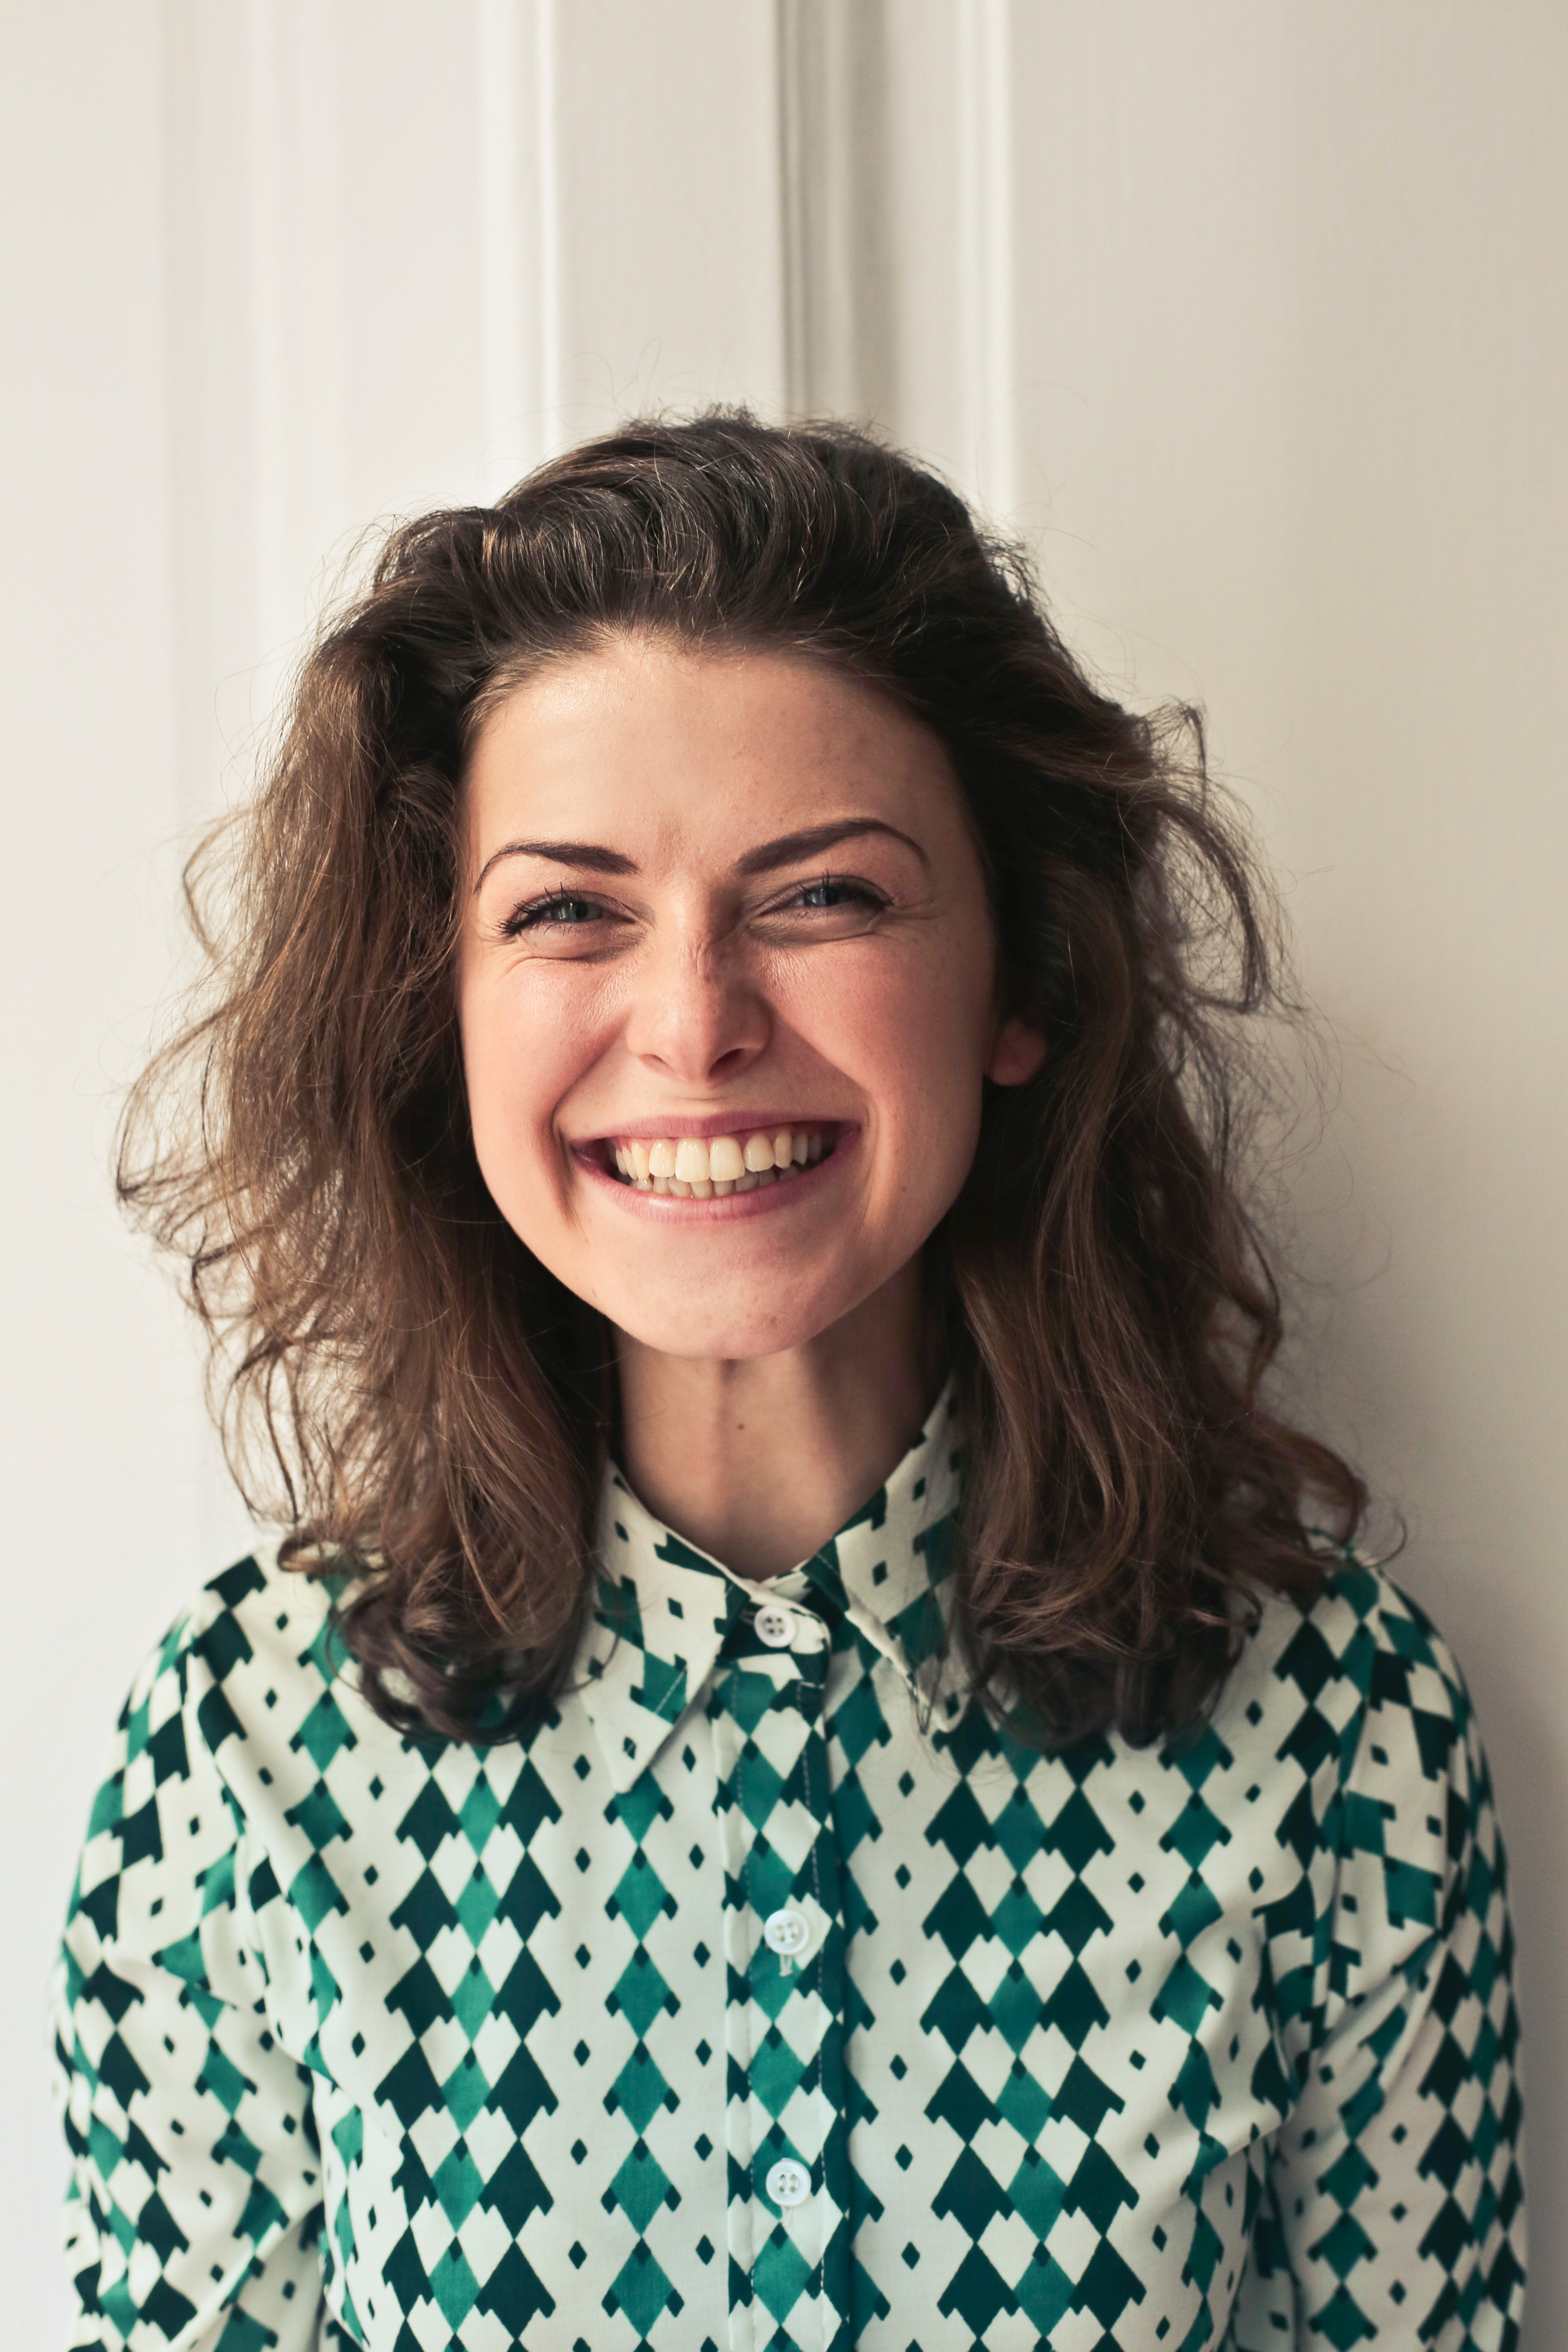
\includegraphics[width=0.80\linewidth, height=1.00\linewidth]{personas/persona_2.jpg}}}
        	\caption{A photo of a fictional female persona for the PyBank application~\cite{PEXELS_FEMALE_PERSONA:4}.}
        	\label{fig:persona_2}
        \end{centering}
    \end{figure}
    \begin{centering}
        \begin{itemize}[leftmargin=*]
            \item {\textbf{Fictional Name:}~Jane Doe}
            \item {\textbf{Job Title:}~Financial Analyst}
            \item {\textbf{Demographics:}
                \begin{itemize}[leftmargin=*]
                    \item {\textbf{Age:}~28}
                    \item {\textbf{Marital Status:}~Married}
                    \item {\textbf{Degree:}~B.A. Finance}
                \end{itemize}
            \item {\textbf{Goals and Tasks:}
                \begin{itemize}[leftmargin=*]
                    \item {Manage personal finances using PyBank's desktop client from the comfort of home.}
                    \item {Utilize PyBank's financial visualizations for insights and reports.}
                \end{itemize}}}
        \end{itemize}
    \end{centering}
\end{minipage}}
\ParallelRText{\begin{minipage}{0.40\textwidth}
    \subsubsection*{Environment}
    \begin{centering}
        Jane is a freelance financial analyst who prefers to work remotely. Her work is generally done on a laptop since she often enjoys working at the coffee shop or other social venues. Jane prefers summarized data visualizations that help her make quick analytical interpretations.
    \end{centering}
    \subsubsection*{Scenario}
    \begin{centering}
        Recently, at Jane's favorite local coffee shop, Jane decided that she wanted to analyzer her families' personal finances and present the results to her husband in an easy to understand manner. With this goal in mind she focused on creating histograms and pie charts for categorical data and a line graph for plotting her families spending over time. With the help of PyBank, she was able to generate these visualizations and produce a summary of her families spending in no time, all while consuming her favorite coffee drink!
        \vspace{43.5mm}
    \end{centering}
\end{minipage}}
\ParallelPar
\end{Parallel}

\newpage

\subsection{Use Case Diagram}
\label{sect:use_case_diagram}

Listed below are brief descriptions of eleven use cases that describe a sequence of a sequence of actions that can be performed by a PyBank customer (the end-user) interacting with PyBank, an interactive desktop client banking application. These use cases are further depicted in Figure~\ref{fig:use_case} shown below after the use case descriptions.

\begin{enumerate}[itemsep=1mm, parsep=0pt]
    % UC_01
    \item {\textbf{CreatePyBankAccount~(UC\_01):}~A PyBank customer can create an account from PyBank's main application window by selecting the~\texttt{\textcolor{red}{Create An Account}}~button.}
    % UC_02
    \item {\textbf{DepositSavingsAccount~(UC\_02):}~A PyBank customer can deposit money into an existing savings account by selecting the~\texttt{\textcolor{red}{Make A Deposit}}~button from the Savings Account application window.}
    % UC_03
    \item {\textbf{DepositCheckingAccount~(UC\_03):}~A PyBank customer can deposit money into an existing checking account by selecting the~\texttt{\textcolor{red}{Make A Deposit}}~button from the Checking Account application window.}
    % UC_04
    \item {\textbf{SignIntoPyBankAccount~(UC\_04):}~A PyBank customer can sign in to an existing account from PyBank's main application window by selecting the~\texttt{\textcolor{red}{Sign In}}~button.}
    % UC_05
    \item {\textbf{WithdrawSavingsAccount~(UC\_05):}~A PyBank customer can withdraw money from an existing savings account by selecting the~\texttt{\textcolor{red}{Make A Withdrawal}}~button from the Savings Account application window.}
    % UC_06
    \item {\textbf{AddCheckingAccount~(UC\_06):}~A PyBank customer can request a checking account from PyBank by selecting the~\texttt{\textcolor{red}{Add A Checking Account}}~button from the main application window. A PyBank customer may have~\textbf{\underline{one}}~checking account per PyBank account.}
    % UC_07
    \item {\textbf{WithdrawCheckingAccount~(UC\_07):}~A PyBank customer can withdraw money from an existing checking account by selecting the~\texttt{\textcolor{red}{Make A Withdrawal}}~button from the Checking Account application window.}
    % UC_08
    \item {\textbf{ViewSavingsAccountGraphs~(UC\_08):}~A PyBank customer can view graphical charts related to their savings account by selecting the~\texttt{\textcolor{red}{View Graphs}}~button from the Savings Account application window.}
    % UC_09
    \item {\textbf{ViewCheckingAccountGraphs~(UC\_09):}~A PyBank customer can view graphical charts related to their checking account by selecting the~\texttt{\textcolor{red}{View Graphs}}~button from the Checking Account application window.}
    % UC_10
    \item {\textbf{AddSavingsAccount~(UC\_10):}~A PyBank customer can request a savings account from PyBank by selecting the~\texttt{\textcolor{red}{Add A Savings Account}}~button from the main application window. A PyBank customer may have~\textbf{\underline{one}}~savings account per PyBank account.}
    % UC_11
    \item {\textbf{SignOutOfPyBankAccount~(UC\_11):}~A PyBank customer can sign out of an existing account from PyBank's main application window by selecting the~\texttt{\textcolor{red}{Sign Out}}~button from the navigation menu.}
\end{enumerate}

\newpage

\begin{figure}[H]
	\begin{centering}
	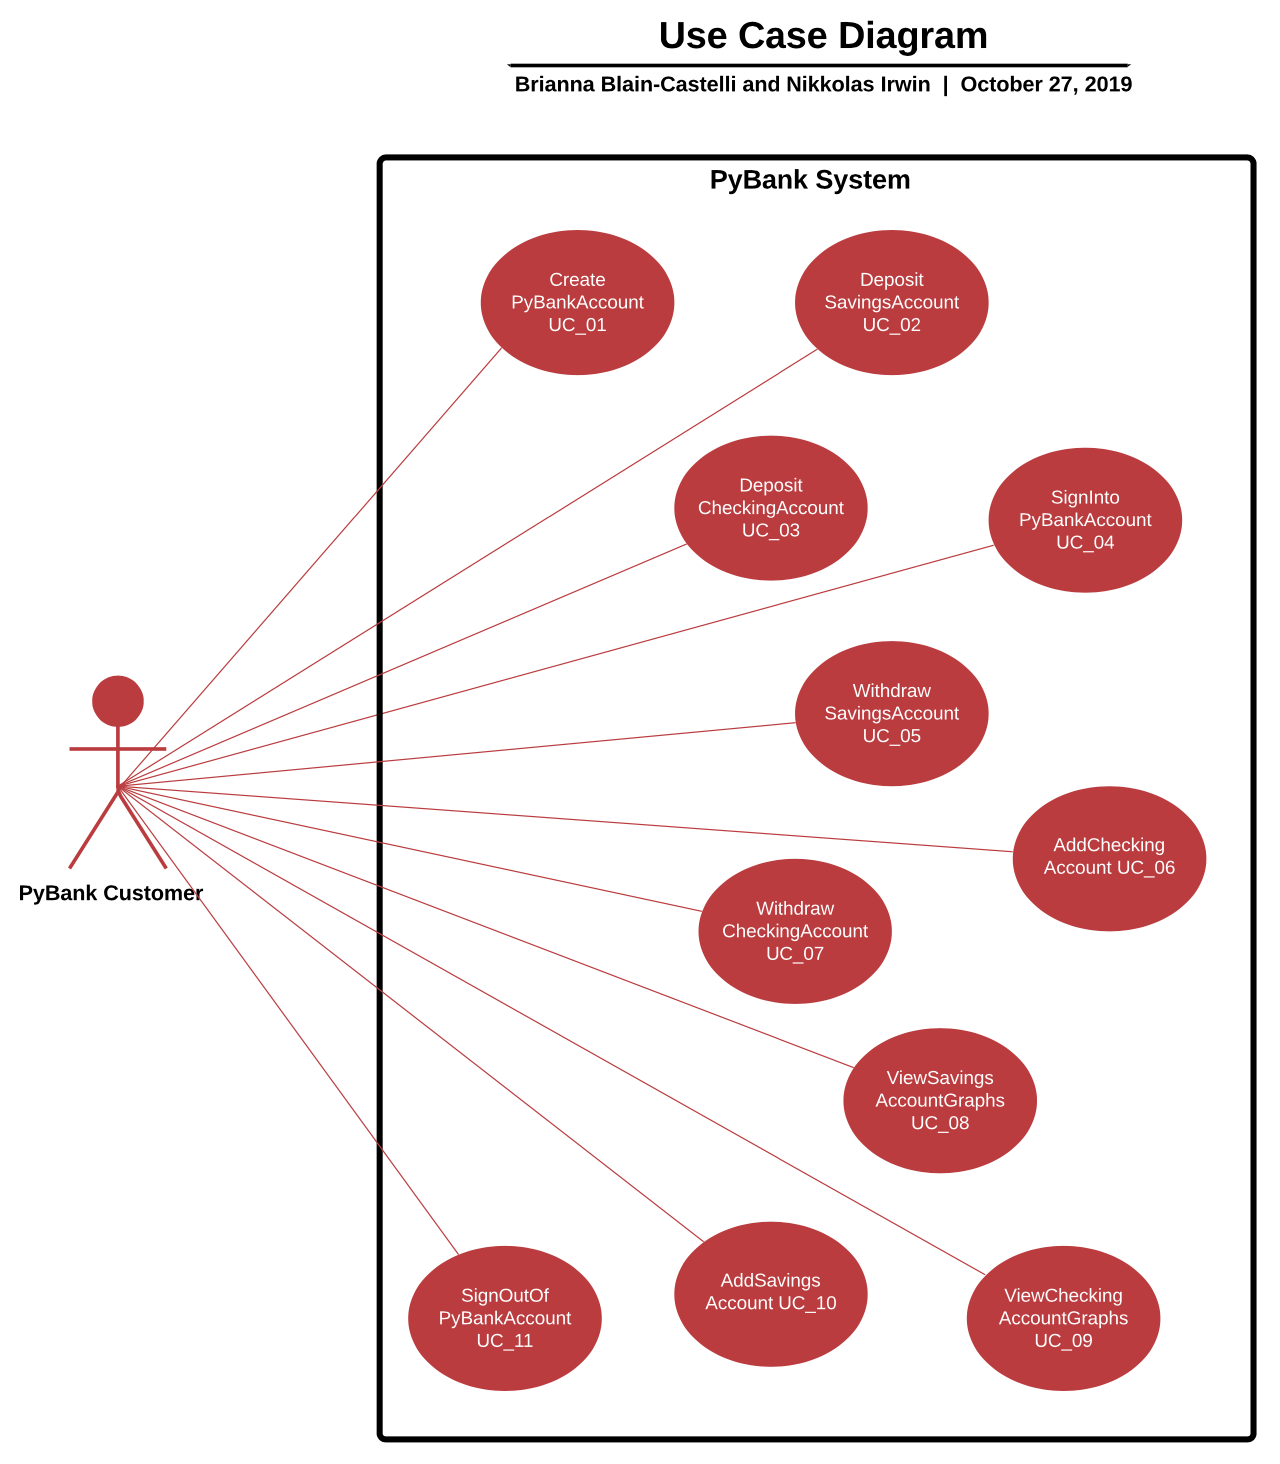
\includegraphics[width=1.00\linewidth, height=1.10\linewidth]{diagrams/use_case_diagram.png}
	\caption{A use case diagram, created using Lucidchart~\cite{LUCID_CHART:5},~for PyBank, an interactive desktop client banking application.}
	\label{fig:use_case}
	\end{centering}
\end{figure}


% EOF
%-----------------------------------END-----OF-----SECTION----------------------------------%
\newpage
%-----------------------------------START-----OF-----SECTION--------------------------------%
\section{Functional Requirements}
\label{sect:functional_requirements}

\subsection{Level 1 Requirements}
\label{sect:level_1_requirements}

Listed below are the level 1 functional requirements which detail functions and features that will be covered in the prototypes interface due in December 2019 and will be fully implemented (from an execution point of view).

\begin{enumerate}[itemsep=1mm, parsep=0pt]
    \item {The system shall provide the end-user access to PyBank through an interactive graphical user interface.}
    \item {The system shall provide an application window for creating a new account or signing into an existing account using text-entry boxes and buttons.}
    \item {The system shall provide username and password checking to verify an end-user's login credentials.}
    \item {The system shall provide the end-user with error dialog windows as feedback for rejected actions.}
    \item {The system shall provide an account overview for an existing user account in the main application window.}
    \item {The system shall provide the end-user with dialog windows as feedback for successful transactions (deposit/withdraw).}
    \item {The system shall request end-user verification before proceeding with any transaction.}
    \item {The system shall provide the ability to request a checking account from the main application window.}
    \item {The system shall provide the ability to view an end-user's checking account from the account overview main application window once signed in.}
    \item {The system shall provide the ability to request a savings account from the main application window.}
    \item {The system shall provide the ability to view an end-user's savings account from the account overview main application window once signed in.}
    \item {The system shall provide various menu options via a menu bar at the top of the main application window.}
    \item {The system shall provide visualizations related to the end-user's checking and spending accounts.}
    \item {The system shall provide the end-user with buttons in their checking and/or savings account(s) to perform actions for depositing and withdrawing money from PyBank.}
\end{enumerate}

\newpage

\subsection{Level 2 Requirements}
\label{sect:level_2_requirements}

Listed below are the level 2 functional requirements which detail functions and features that will be covered in the prototype's interface due in December 2019 but will not be fully implemented.

\begin{enumerate}[itemsep=1mm, parsep=0pt]
    \item {The system shall provide the ability to transfer funds to other PyBank customers.}
    \item {The system shall provide a `switch theme' menu option.}
    \item {The system shall provide the ability to request a credit card account.}
    \item {The system shall provide the ability to view an end-user's credit card account from the account overview main application window once signed in.}
    \item {The system shall provide a `help' menu option.}
\end{enumerate}

\subsection{Level 3 Requirements}
\label{sect:level_3_requirements}

Listed below are the level 3 functional requirements which detail functions and features that will not be covered in the prototype due in December 2019 but would be useful in a possible continuation of the project beyond the time frame of this course.

\begin{enumerate}[itemsep=1mm, parsep=0pt]
    \item {The system shall use modern encryption techniques to protect the account creation and sign-in processes.}
    \item {The system shall provide advanced visualizations and using statistical techniques.}
    \item {The system shall add additional options for customizing the applications interface.}
    \item {The system shall provide predictive models based on spending trends.}
    \item {The system shall provide the end-user with detailed reports related to their existing accounts.}
\end{enumerate}

% EOF
%-----------------------------------END-----OF-----SECTION----------------------------------%
\newpage
%-----------------------------------START-----OF-----SECTION--------------------------------%
\phantomsection
\addcontentsline{toc}{section}{References}
\label{sect:references}
\bibliography{main.bib}
\bibliographystyle{ieeetr}

% EOF
%-----------------------------------END-----OF-----SECTION----------------------------------%

\end{document}

% EOF